% Chapter 2

\chapter{Literature review}

\section{Literature Review Introduction}

Starting of text

\begin{itemize}
\item Bullet (single spacing)
\item Bullet
\item Bullet
\end{itemize}

Figures comprise photographs, diagrams, graphs, bar charts, pie charts, etc. They are all termed ``Figures'', and are captioned \underline{below the figure} (Microsoft Word: Insert -- Reference -- Caption). If the caption is longer than one line, it should be typed in \underline{single line-spacing}. Figures taken (or adapted) from a source should be acknowledged as in the example below, and should appear in the Bibliography/References. Leave at least two spaces (press enter twice) above and below a figure, to separate it from the text.

% Example figure
\begin{figure}[htbp]
\centering
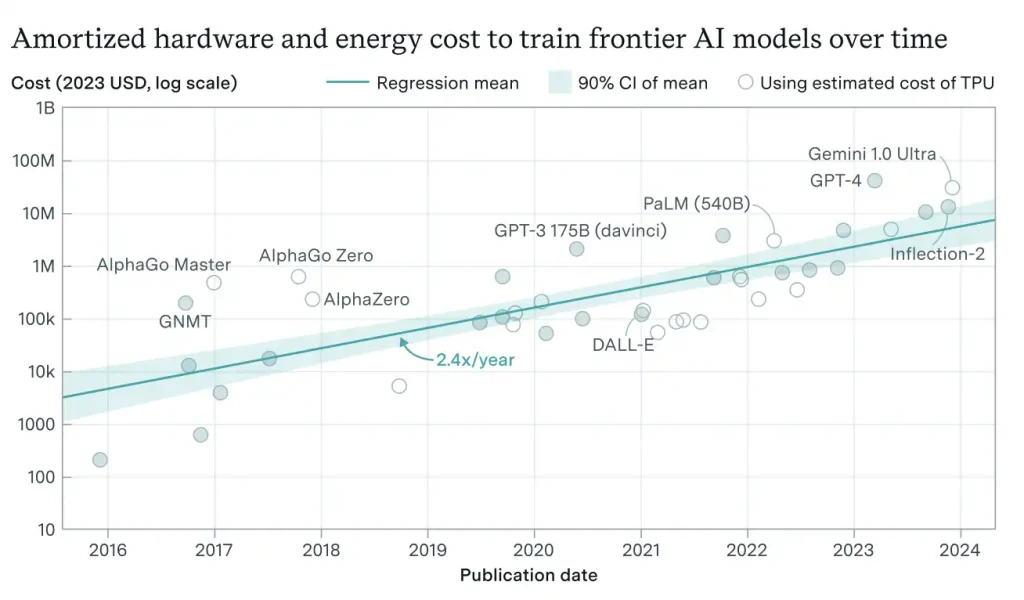
\includegraphics[width=0.8\textwidth]{media/Fig1.png}
\caption{Example figure}
\label{fig:2.1}
\end{figure}

Tables comprise text and figures in tabular form. Tables are typed in single line-spacing, with left justification. Figures should be aligned to the right, as in the example below. If you have a great deal of text, use a smaller (but legible) font, e.g. 9- or 10-point. Acknowledge tables taken from another source as for figures, above. Leave at least two spaces (press enter twice) above and below a table, to separate it from the text.

% Example table
\begin{table}[htbp]
\centering
\caption{Example table}
\begin{tabularx}{0.86\textwidth}{|Y|Y|Y|Y|>{\raggedleft\arraybackslash}p{1.8cm}|}
\hline
\textbf{Column 1} & \textbf{Column 2} & \textbf{Column 3} & \textbf{Column 4} & \textbf{Value} \\
\hline
Data 1 & Data 2 & Data 3 & Data 4 & 123.45 \\
\hline
Data 5 & Data 6 & Data 7 & Data 8 & 678.90 \\
\hline
\end{tabularx}
\label{tab:2.1}
\end{table}
